\documentclass[12pt, a4paper]{article}
% Suppress reference warnings
\usepackage{silence}
\WarningFilter*{}{Label}

\usepackage{vntex}
\usepackage[dvipsnames]{xcolor}
%\usepackage[english,vietnam]{babel}
%\usepackage[utf8]{inputenc}

%\usepackage[utf8]{inputenc}
%\usepackage[francais]{babel}
\usepackage{a4wide,amssymb,epsfig,latexsym,array,hhline,fancyhdr}
\usepackage[normalem]{ulem}
%\usepackage{soul}
\usepackage{caption}
\usepackage{float}
\renewcommand{\figurename}{}
\usepackage{wasysym}
\usepackage{enumitem}
\usepackage[makeroom]{cancel}
\let\iint\relax
\let\iiint\relax
\usepackage{amsmath}
\usepackage{amsfonts}
\usepackage{amssymb}
\usepackage{amsthm}
\usepackage{multicol,longtable,amscd}
\usepackage{diagbox}%Make diagonal lines in tables
\usepackage{booktabs}
\usepackage{alltt}
\usepackage[framemethod=tikz]{mdframed}% For highlighting paragraph backgrounds
\usepackage{caption,subcaption}
\usepackage{listings}
\usepackage{color}
\usepackage[lined,boxed,commentsnumbered]{algorithm2e}
\usepackage{enumerate}
\usepackage{graphicx}
\usepackage{array}
\usepackage{tabularx, caption}
\usepackage{multirow}
\usepackage{multicol}
\usepackage{rotating}
\usepackage{graphics}
\usepackage{geometry}
\usepackage{setspace}
\usepackage{epsfig}
\usepackage{tikz}
\usepackage[colorlinks=true, linkcolor=blue, urlcolor=blue, unicode]{hyperref}
\usetikzlibrary{arrows,snakes,backgrounds}

\hypersetup{urlcolor=blue,linkcolor=black,citecolor=black,colorlinks=true} 
%\usepackage{pstcol} % PSTricks with the standard color package

\newcolumntype{P}[1]{>{\centering\arraybackslash}p{#1}}

\newcolumntype{M}[1]{>{\centering\arraybackslash}m{#1}}

\newtheorem{theorem}{{\bf Định lý}}

\newtheorem{property}{{\bf Tính chất}}
\newtheorem{proposition}{{\bf Mệnh đề}}
\newtheorem{corollary}[proposition]{{\bf Hệ quả}}
\newtheorem{lemma}[proposition]{{\bf Bổ đề}}
\theoremstyle{definition}
\newtheorem{exer}{Bài toán}

\def\thesislayout{	% A4: 210 × 297
	\geometry{
		a4paper,
		total={160mm,240mm},  % fix over page
		left=30mm,
		top=30mm,
	}
}
\thesislayout%

%\usepackage{fancyhdr}
\setlength{\headheight}{40pt}
\pagestyle{fancy}
\fancyhead{} % clear all header fields
\fancyhead[L]{
 \begin{tabular}{rl}
    %\begin{picture}(25,15)(0,0)
    %\put(0,-8){\includegraphics[width=8mm, height=8mm]{hcmut.png}}
    %\put(0,-8){\epsfig{width=10mm,figure=hcmut.eps}}
   %\end{picture}&
	%\includegraphics[width=8mm, height=8mm]{hcmut.png} & %
	\begin{tabular}{l}
		\textbf{\bf \ttfamily Trường Đại Học Bách Khoa \textendash{} ĐHQG TP.HCM}\\
		\textbf{\bf \ttfamily Khoa Kỹ thuật và Khoa học Máy tính}
	\end{tabular} 	
 \end{tabular}
}
\fancyhead[R]{
	\begin{tabular}{l}
		\tiny \bf \\
		\tiny \bf 
	\end{tabular}  }
\fancyfoot{} % clear all footer fields
\fancyfoot[L]{\scriptsize \ttfamily Báo cáo bài tập lớn Vật lý Bán dẫn \textendash{} EE$1007$ \\ Niên khoá 2024 \textendash{} 2025}
\makeatletter
\fancyfoot[R]{\scriptsize \ttfamily Trang {\thepage}/\@ifundefined{r@LastPage}{?}{\pageref{LastPage}}}
\makeatother
\renewcommand{\headrulewidth}{0.3pt}
\renewcommand{\footrulewidth}{0.3pt}
%%%
\setcounter{secnumdepth}{4}
\setcounter{tocdepth}{3}
\makeatletter
\newcounter{subsubsubsection}[subsubsection]
\renewcommand\thesubsubsubsection{\thesubsubsection.\@alph\c@subsubsubsection}
\newcommand\subsubsubsection{\@startsection{subsubsubsection}{4}{\z@}%
                                     {-3.25ex\@plus -1ex \@minus -.2ex}%
                                     {1.5ex \@plus .2ex}%
                                     {\normalfont\normalsize\bfseries}}
\newcommand*\l@subsubsubsection{\@dottedtocline{3}{10.0em}{4.1em}}
\newcommand*{\subsubsubsectionmark}[1]{}
\makeatother

\everymath{\color{black}}%make in-line maths symbols blue to read/check easily

\sloppy
%\captionsetup[figure]{labelfont={small,bf},textfont={small,it},belowskip=-1pt,aboveskip=-9pt}
%space remove between caption, figure, and text
%\captionsetup[table]{labelfont={small,bf},textfont={small,it},belowskip=-1pt,aboveskip=7pt}
%space remove between caption, table, and text

%\floatplacement{figure}{H}%forced here float placement automatically for figures
%\floatplacement{table}{H}%forced here float placement automatically for table
%the following settings (11 lines) are to remove white space before or after the figures and tables
%\setcounter{topnumber}{2}
%\setcounter{bottomnumber}{2}
%\setcounter{totalnumber}{4}
%\renewcommand{\topfraction}{0.85}
%\renewcommand{\bottomfraction}{0.85}
%\renewcommand{\textfraction}{0.15}
%\renewcommand{\floatpagefraction}{0.8}
%\renewcommand{\textfraction}{0.1}
\setlength{\floatsep}{5pt plus 2pt minus 2pt}
\setlength{\textfloatsep}{5pt plus 2pt minus 2pt}
\setlength{\intextsep}{10pt plus 2pt minus 2pt}

\thesislayout%
% chktex 1 off
% chktex 8 off
\lstset{
language=C++,
    aboveskip=6mm,
    belowskip=-6mm,
    backgroundcolor=\color{white},   
    commentstyle=\color{codegreen},
    keywordstyle=\color{blue},
    numberstyle=\tiny\color{codegray},
    stringstyle=\color{codepurple},
    basicstyle=\ttfamily,
    breakatwhitespace=false,         
    breaklines=true,                 
    captionpos=b,                    
    keepspaces=true,                 
    numbers=left,                    
    numbersep=5pt,                  
    showspaces=false,                
    showstringspaces=false,
    showtabs=false,                  
    tabsize=2,
    frame=tb,
    framesep=8pt,
    rulecolor=\color{black},
    title=\lstname,
}

\usepackage{listings}

\usepackage{xcolor}

%New colors defined below
\definecolor{codegreen}{rgb}{0,0.6,0}
\definecolor{codegray}{rgb}{0.5,0.5,0.5}
\definecolor{codepurple}{rgb}{0.58,0,0.82}
\definecolor{backcolour}{rgb}{0.95,0.95,0.92}

%Code listing style named "mystyle"
\lstdefinestyle{mystyle}{
  backgroundcolor=\color{backcolour}, commentstyle=\color{codegreen},
  keywordstyle=\color{magenta},
  numberstyle=\tiny\color{codegray},
  stringstyle=\color{codepurple},
  basicstyle=\ttfamily\footnotesize,
  breakatwhitespace=false,         
  breaklines=true,                 
  captionpos=b,                    
  keepspaces=true,                 
  numbers=left,                    
  numbersep=5pt,                  
  showspaces=false,                
  showstringspaces=false,
  showtabs=false,                  
  tabsize=2
}

%"mystyle" code listing set
\lstset{style=mystyle}
\lstset{
        literate=%
% Vần a
	{á}{{\'a}}1
	{à}{{\`a}}1
	{ạ}{{\d a}}1
	{ả}{{\h a}}1
	{ã}{{\~ a}}1
	%
	{Á}{{\'A}}1
	{À}{{\`A}}1
	{Ạ}{{\d A}}1
	{Ả}{{\h A}}1
	{Ã}{{\~ A}}1
%
% Vần ă
	{ă}{{\u a}}1
	{ắ}{{\'\abreve }}1
	{ằ}{{\`\abreve }}1
	{ặ}{{\d \abreve }}1
	{ẳ}{{\h \abreve }}1
	{ẵ}{{\~\abreve }}1
	%
	{Ă}{{\u A}}1
	{Ắ}{{\'\ABREVE }}1
	{Ằ}{{\`\ABREVE }}1
	{Ặ}{{\d \ABREVE }}1
	{Ẳ}{{\h \ABREVE }}1
	{Ẵ}{{\~\ABREVE }}1
%
% Vần â
	{â}{{\^ a}}1
	{ấ}{{\'\acircumflex }}1
	{ầ}{{\`\acircumflex }}1
	{ậ}{{\d \acircumflex }}1
	{ẩ}{{\h \acircumflex }}1
	{ẫ}{{\~\acircumflex }}1
	 %
	{Â}{{\^ A}}1
	{Ấ}{{\'\ACIRCUMFLEX }}1
	{Ầ}{{\`\ACIRCUMFLEX }}1
	{Ậ}{{\d \ACIRCUMFLEX }}1
	{Ẩ}{{\h \ACIRCUMFLEX }}1
	{Ẫ}{{\~\ACIRCUMFLEX }}1
%
% Vần đ
	{đ}{{\dj }}1
	{Đ}{{\DJ }}1
%
% Vần e
	{é}{{\'e}}1
	{è}{{\`e}}1
	{ẹ}{{\d e}}1
	{ẻ}{{\h e}}1
	{ẽ}{{\~ e}}1
	%
	{É}{{\'E}}1
	{È}{{\`E}}1
	{Ẹ}{{\d E}}1
	{Ẻ}{{\h E}}1
	{Ẽ}{{\~ E}}1
%
% Vần ê
	{ê}{{\^e}}1
	{ế}{{\'\ecircumflex }}1
	{ề}{{\`\ecircumflex }}1
	{ệ}{{\d \ecircumflex }}1
	{ể}{{\h \ecircumflex }}1
	{ễ}{{\~\ecircumflex }}1
	%
	{Ê}{{\^E}}1
	{Ế}{{\'\ECIRCUMFLEX }}1
	{Ề}{{\`\ECIRCUMFLEX }}1
	{Ệ}{{\d \ECIRCUMFLEX }}1
	{Ể}{{\h \ECIRCUMFLEX }}1
	{Ễ}{{\~\ECIRCUMFLEX }}1
%
% Vần i
	{í}{{\'i}}1
	{ì}{{\`\i }}1
	{ị}{{\d i}}1
	{ỉ}{{\h i}}1
	{ĩ}{{\~\i }}1
	%
	{Í}{{\'I}}1
	{Ì}{{\`I}}1
	{Ị}{{\d I}}1
	{Ỉ}{{\h I}}1
	{Ĩ}{{\~I}}1
%
% Vần o
	{ó}{{\'o}}1
	{ò}{{\`o}}1
	{ọ}{{\d o}}1
	{ỏ}{{\h o}}1
	{õ}{{\~o}}1
	%
	{Ó}{{\'O}}1
	{Ò}{{\`O}}1
	{Ọ}{{\d O}}1
	{Ỏ}{{\h O}}1
	{Õ}{{\~O}}1
%
% Vần ô
	{ô}{{\^o}}1
	{ố}{{\'\ocircumflex }}1
	{ồ}{{\`\ocircumflex }}1
	{ộ}{{\d \ocircumflex }}1
	{ổ}{{\h \ocircumflex }}1
	{ỗ}{{\~\ocircumflex }}1
	%
	{Ô}{{\^O}}1
	{Ố}{{\'\OCIRCUMFLEX }}1
	{Ồ}{{\`\OCIRCUMFLEX }}1
	{Ộ}{{\d \OCIRCUMFLEX }}1
	{Ổ}{{\h \OCIRCUMFLEX }}1
	{Ỗ}{{\~\OCIRCUMFLEX }}1
%
% Vần ơ
	{ơ}{{\ohorn }}1
	{ớ}{{\'\ohorn }}1
	{ờ}{{\`\ohorn }}1
	{ợ}{{\d \ohorn }}1
	{ở}{{\h \ohorn }}1
	{ỡ}{{\~\ohorn }}1
	%
	{Ơ}{{\OHORN }}1
	{Ớ}{{\'\OHORN }}1
	{Ờ}{{\`\OHORN }}1
	{Ợ}{{\d \OHORN }}1
	{Ở}{{\h \OHORN }}1
	{Ỡ}{{\~\OHORN }}1
%
% Vần u
	{ú}{{\'u}}1
	{ù}{{\`u}}1
	{ụ}{{\d u}}1
	{ủ}{{\h u}}1
	{ũ}{{\~u}}1
	%
	{Ú}{{\'U}}1
	{Ù}{{\`U}}1
	{Ụ}{{\d U}}1
	{Ủ}{{\h U}}1
	{Ũ}{{\~U}}1
%
% Vần ư
	{ư}{{\uhorn }}1
	{ứ}{{\'\uhorn }}1
	{ừ}{{\`\uhorn }}1
	{ự}{{\d \uhorn }}1
	{ử}{{\h \uhorn }}1
	{ữ}{{\~\uhorn }}1
	%
	{Ư}{{\UHORN }}1
	{Ứ}{{\'\UHORN }}1
	{Ừ}{{\`\UHORN }}1
	{Ự}{{\d \UHORN }}1
	{Ử}{{\h \UHORN }}1
	{Ữ}{{\~\UHORN }}1
%
% Vần y
	{ý}{{\'y}}1
	{ỳ}{{\`y}}1
	{ỵ}{{\d y}}1
	{ỷ}{{\h y}}1
	{ỹ}{{\~y}}1
	%
	{Ý}{{\'Y}}1
	{Ỳ}{{\`Y}}1
	{Ỵ}{{\d Y}}1
	{Ỷ}{{\h Y}}1
	{Ỹ}{{\~Y}}1
}
% chktex 1 on
% chktex 8 on

\newmdenv[linecolor=black,skipabove=10pt,skipbelow=0pt,innertopmargin=5pt,innerbottommargin=5pt
leftmargin=-5pt,rightmargin=-5pt,
innerleftmargin=40pt,innerrightmargin=40pt]{mybox1}
\newmdenv[linecolor=black,skipabove=\topsep,skipbelow=\topsep,innertopmargin=20pt,innerbottommargin=10pt
leftmargin=-5pt,rightmargin=-5pt,
innerleftmargin=20pt,innerrightmargin=40pt]{mybox}



\begin{document}
\begin{titlepage}
   \begin{tikzpicture}[remember picture,overlay,inner sep=0,outer sep=0]
     \draw[blue!70!black,line width=4pt] ([xshift=-1.5cm,yshift=-2cm]current page.north east) coordinate (A)--([xshift=2.4cm,yshift=-2cm]current page.north west) coordinate(B)--([xshift=2.4cm,yshift=2cm]current page.south west) coordinate (C)--([xshift=-1.5cm,yshift=2cm]current page.south east) coordinate(D)--cycle;

     \draw ([yshift=0.5cm,xshift=-0.5cm]A)-- ([yshift=0.5cm,xshift=0.5cm]B)--
     ([yshift=-0.5cm,xshift=0.5cm]B) --([yshift=-0.5cm,xshift=-0.5cm]B)--([yshift=0.5cm,xshift=-0.5cm]C)--([yshift=0.5cm,xshift=0.5cm]C)--([yshift=-0.5cm,xshift=0.5cm]C)-- ([yshift=-0.5cm,xshift=-0.5cm]D)--([yshift=0.5cm,xshift=-0.5cm]D)--([yshift=0.5cm,xshift=0.5cm]D)--([yshift=-0.5cm,xshift=0.5cm]A)--([yshift=-0.5cm,xshift=-0.5cm]A)--([yshift=0.5cm,xshift=-0.5cm]A);

     \draw ([yshift=-0.3cm,xshift=0.3cm]A)-- ([yshift=-0.3cm,xshift=-0.3cm]B)--
     ([yshift=0.3cm,xshift=-0.3cm]B) --([yshift=0.3cm,xshift=0.3cm]B)--
     ([yshift=-0.3cm,xshift=0.3cm]C)--([yshift=-0.3cm,xshift=-0.3cm]C)--([yshift=0.3cm,xshift=-0.3cm]C)-- ([yshift=0.3cm,xshift=0.3cm]D)--([yshift=-0.3cm,xshift=0.3cm]D)--([yshift=-0.3cm,xshift=-0.3cm]D)--([yshift=0.3cm,xshift=-0.3cm]A)--([yshift=0.3cm,xshift=0.3cm]A)--([yshift=-0.3cm,xshift=0.3cm]A);

   \end{tikzpicture}

\begin{center}
\vspace*{-0.8cm}
{\textbf{\large ĐẠI HỌC QUỐC GIA THÀNH PHỐ HỒ CHÍ MINH}} \\
{\textbf{\large TRƯỜNG ĐẠI HỌC BÁCH KHOA}} \\
{\textbf{\large KHOA KỸ THUẬT VÀ KHOA HỌC MÁY TÍNH}}
\end{center}

\vspace{0.3cm}

\begin{center}
\includegraphics[scale=0.15]{images/Logo BK.png}
\end{center}

\vspace{0.2cm}

\begin{center}
{\textbf{\Large BÁO CÁO BÀI TẬP LỚN}}\\[0.2cm]
{\textbf{\large GIẢI TÍCH 1 - MT1003}}\\[0.2cm]
{\textbf{\large ĐỀ TÀI: VI PHÂN TUYẾN TÍNH CẤP 1}}\\[0.2cm]
{\textbf{\large GVHD: THS. ĐÀO THỊ THANH XUÂN}}\\[0.2cm]
{\textbf{\large NHÓM 05 -- LỚP CN02KHM1 -- HK251}}
\end{center}

\vspace{0.2cm}

\begin{center}
{\textbf{DANH SÁCH THÀNH VIÊN}}\\[0.15cm]
{\small
\begin{tabular}{|c|c|c|c|c|}
\hline
\textbf{STT} & \textbf{Họ và Tên} & \textbf{MSSV} & \textbf{Điểm số} & \textbf{Chữ ký} \\
\hline
1 & Dương Gia Bảo & 2410611 & & \\
\hline
2 & Đinh Nhật Huy & 2410824 & & \\
\hline
3 & Phạm Thái Duy Bảo & 2411715 & & \\
\hline
4 & Trần Tuấn Kiệt & 2410821 & & \\
\hline
5 & Trần Thái Hòa & 2551895 & & \\
\hline
6 & Nguyễn Hoàng Minh Khang & 2551900 & & \\
\hline
7 & Đặng Nguyễn Thiên Phúc & 2551919 & & \\
\hline
8 & Cao Lê Khiết & 2551902 & & \\
\hline
\end{tabular}
}
\end{center}

\vspace{0.3cm}

\begin{center}
{\large TP. Hồ Chí Minh, tháng 11 năm 2025}
\end{center}
\end{titlepage}
\newpage
\tableofcontents
\newpage
\begin{center}
\scalebox{2}{\textcolor{blue}{LỜI CẢM ƠN}} \\[0.5cm]
\end{center}
{
\Large % <-- LỆNH TĂNG KÍCH THƯỚC CHỮ (Bạn có thể dùng \huge hoặc \Huge)
\sloppy % <-- LỆNH CHỐNG TRÀN LỀ (Nới lỏng quy tắc ngắt dòng)

\textit{Đầu tiên, chúng em xin cảm ơn khoa Kỹ thuật và Khoa học Máy tính,
Trường Đại học Bách khoa - Đại học Quốc gia TP.HCM đã đưa
bộ môn Giải tích 1 vào chương trình giảng dạy và kế hoạch học
tập của chúng em, trong thời gian học môn này, chúng em đã
học được rất nhiều kiến thức bổ ích, thiết thực trong thực tế
cũng như cho quá trình học tập sau này của chúng em. Chúng
em cũng xin gửi lời cảm ơn đến cô Đào Thị Thanh Xuân đã tận
tình giảng dạy trong thời gian học tập trên lớp của cô quả thực rất
chất lượng và góp phần rất lớn trong quá trình giúp chúng em
hoàn thành bài báo cáo bài tập lớn lần này.}
\par
\textit{Tuy nhiên, vì vốn kiến thức còn hạn hẹp cũng như khả năng
vận dụng còn hạn chế nên chúng em không thể tránh khỏi
những sai sót không đáng có trong quá trình thực hiện bài tập
cũng như soạn nên bài báo cáo này. Vì vậy chúng em cũng
kính mong cô xem xét, đánh giá và góp ý để chúng em có
thể thực hiện tốt hơn ở các bài tập lớn sau.
Chúng em xin trân trọng cảm ơn.}

} % Kết thúc nhóm, kích thước chữ và chế độ ngắt dòng trở về mặc định
\newpage
\begin{center}
\scalebox{2}{\textcolor{blue}{NỘI DUNG CHÍNH}} \\[0.5cm]
\end{center}
\vspace{0.6cm}

\section{\bfseries Khái niệm phương trình vi phân cấp 1.}\par
\subsection{\bfseries Khái niệm phương trình vi phân cấp 1.}
\indent\hspace{0.4cm} Phương trình vi phân là phương trình chứa đạo hàm cấp 1 hoặc vi phân cấp 1 của 1 hoặc vài hàm cần tìm.

Dạng tổng quát của phương trình vi phân cấp 1 là: 
\[ F(x,y,y') = 0\]

\subsection{\bfseries Nghiệm tổng quát.}
\indent\hspace{0.4cm} 
Nghiệm tổng quát của của phương trình vi phân cấp một \( F(x, y, y') = 0 \) là biểu thức tổng quát của tập hợp vô hạn các hàm, thỏa mãn phương trình vi phân. Có thể được xác định ở dạng tường minh \( y = F(x,C)\) hoặc dạng ẩn \( \Phi(x, y, C) = 0 \) với \( C \) là hằng số tùy ý.
\par
Nghiệm của phương trình vi phân tương ứng với một giá trị C cụ thể được gọi là nghiệm riêng. Nghiệm của phương trình vi phân không tương ứng với một giá C cụ nào được gọi là nghiệm kỳ dị. Thường xuất hiện ở điểm đặc biệt hoặc giới hạn của nghiệm tổng quát.
\subsection{\bfseries Phương trình vi phân cấp 1.}
\indent\hspace{0.5cm}
Phương trình vi phân có dạng:
\[
y' + P(x)y = Q(x), \quad y' = \frac{dy}{dx}
\]
\indent\hspace{0cm}
Gọi là phương trình vi phân tuyến tính cấp một. Trong đó \( P(x)y \) và \( Q(x) \) là các hàm liên tục.

\vspace{0.3cm}
\indent\hspace{0.2cm}
Nếu \( Q(x) = 0 \) thì phương trình được gọi là \textbf{phương trình thuần nhất}.

\vspace{0.3cm}
\indent\hspace{0.2cm}
Nếu \( Q(x) \ne 0 \) thì phương trình được gọi là \textbf{phương trình không thuần nhất}
.
\section{ Phương pháp giải.}
\subsection{Phương pháp giải.}
\begin{itemize}
    \item[] \textbf{Bước 1:} Tìm biểu thức \( A(x) = e^{-\int P(x)\,dx} \).
    \item[] \textbf{Bước 2:} Tìm biểu thức \( B(x) = \int \frac{Q(x)}{A(x)}\,dx \).
    \item[] \textbf{Bước 3:} Nghiệm tổng quát là \( y = A(x)[B(x) + C] \).
\end{itemize}
\subsection{Ví dụ.}
\indent\hspace{0.4cm}
Giải phương trình \( y' + \frac{1}{x}y = 3x \) với điều kiện \( y(1) = 1 \).

\vspace{0.3cm}
Ta có:
\[
P(x) = \frac{1}{x}, \quad Q(x) = 3x
\]

\vspace{0.3cm}
Tính:
\[
A(x) = e^{-\int P(x)\,dx} = e^{-\int \frac{1}{x}\,dx} = \frac{1}{x}
\]

\[
B(x) = \int \frac{Q(x)}{A(x)}\,dx = \int 3x \cdot x\,dx = \int 3x^2\,dx = x^3
\]

\vspace{0.3cm}
Nghiệm tổng quát:
\[
y = A(x)[B(x) + C] = \frac{1}{x}(x^3 + C)
\]

\vspace{0.3cm}
Áp dụng điều kiện ban đầu \( x = 1, y = 1 \):
\[
1 = \frac{1}{1}(1^3 + C) \Rightarrow C = 0
\]

\vspace{0.3cm}
Vậy nghiệm của phương trình đã cho là:
\[
y = x^2
\]
\section{\bfseries Bài toán lãi suất đưa về phương trình vi phân tuyến tính cấp 1.}
\subsection{\bfseries Lý thuyết.}
\indent\hspace{0.4cm}
Giả sử số tiền \( A(t) \) tăng trưởng theo lãi suất liên tục \( r \) trong khoảng thời gian rất nhỏ \( dt \). Khi đó, số tiền tăng thêm là:

\[
dA = rA(t)\,dt
\]

Giả sử có thêm một hàm \( f(t) \) biểu diễn dòng tiền vào hoặc ra tại thời điểm \( t \). Khi đó, phương trình vi phân mô tả sự thay đổi của số tiền là:

\[
\frac{dA}{dt} = rA(t) - f(t)
\]

Tương đương, ta có phương trình vi phân tuyến tính cấp một không thuần nhất:

\[
A'(t) - rA(t) = -f(t)
\]
\subsection{ Dạng tổng quát.}
\indent\hspace{0.4cm}
Phương trình vi phân tuyến tính cấp một có dạng:
\[
y'(t) + P(t)y(t) = Q(t)
\]

Trong bài toán tài chính, ta có:
\begin{itemize}
    \item \( y(t) = A(t) \): số tiền hoặc số dư nợ
    \item \( P(t) = -r \): hệ số lãi suất (hằng số hoặc hàm theo thời gian)
    \item \( Q(t) = -f(t) \): dòng tiền vào/ra
\end{itemize}

Do đó, mọi bài toán lãi suất liên tục đều đưa về dạng tuyến tính cấp một.

\subsection{Phương pháp giải.}
\indent\hspace{0.4cm}
Xét phương trình:
\[
A'(t) - rA(t) = -f(t)
\]

Nhân cả hai vế của phương trình với nhân tử tích phân \( e^{\int P(t)\,dt} = e^{-rt} \), ta được:
\[
e^{-rt}A'(t) - re^{-rt}A(t) = -f(t)e^{-rt}
\]

Nhận thấy vế trái là đạo hàm của tích:
\[
(A(t)e^{-rt})' = -f(t)e^{-rt}
\]

Lấy tích phân hai vế:
\[
A(t)e^{-rt} = -\int f(t)e^{-rt}\,dt + C
\]

Suy ra nghiệm tổng quát:
\[
A(t) = e^{rt}\left(C - \int f(t)e^{-rt}\,dt\right)
\]
\section{Các dạng bài toán lãi suất}
\indent\hspace{0.4cm}
Giả sử \( f(t) \) là một hằng số \( K \).

Điều kiện ban đầu:
\[
A(0) = e^{rt} \left( C - \int f(t)e^{-rt} \, dt \right) = Ce^{r \cdot 0} = \frac{e^{r \cdot 0} K}{e^{r \cdot 0} r} = C - \frac{K}{r}
\]

Suy ra:
\[
C = A(0) + \frac{K}{r}
\]

\subsection{Trả góp đều / Rút tiền đều}
\indent\hspace{0.4cm}
Với \( f(t) = K \), ta có phương trình vi phân:
\[
A'(t) = rA(t) - K
\]

Nghiệm tổng quát:
\[
A(t) = \frac{K}{r} + \left( A_0 - \frac{K}{r} \right) e^{rt}
\]
\subsection{Gửi tiền đều}
\indent\hspace{0.4cm}
Nếu mỗi tháng hoặc mỗi năm gửi vào ngân hàng một khoản đều đặn \( K \), ta có phương trình vi phân:

\[
A'(t) = rA(t) + K
\]

Nghiệm tổng quát của phương trình là:

\[
A(t) = -\frac{K}{r} + \left( A_0 + \frac{K}{r} \right) e^{rt}
\]

\vspace{0.5cm}
\subsection{Không gửi/rút thêm}
\indent\hspace{0.4cm}
Khi \( f(t) = 0 \), tức là không có dòng tiền vào hoặc ra, ta có phương trình:

\[
A'(t) = rA(t)
\]

Nghiệm tổng quát:

\[
A(t) = A(0) \cdot e^{rt}
\]





\end{document}
